\documentclass{beamer}
\hypersetup{pdfpagemode=FullScreen}
\usepackage{fontspec}
\usepackage{tcolorbox}
\tcbuselibrary{minted,skins}
\usepackage{graphicx}
\graphicspath{ {./images/} }

\newtcblisting{bashcode}{
  listing engine=minted,
  colback=bashcodebg,
  colframe=bashcodebg,
  listing only,
  minted style=native,
  minted language=bash,
  minted options={linenos=true,texcl=true},
  left=1mm,
}
\definecolor{bashcodebg}{rgb}{0.95,0.95,0.95}

\setsansfont{Open Sans}

\usetheme{metropolis}           % Use metropolis theme
\title{Lesson 1: React Native Basics}
\subtitle{and how to get started!}
\date{\today}
\author{Karl Steven Velasco Orjalo}
\institute{React Native Quickstart}

\begin{document}
\metroset{block=fill}
  \maketitle

  \begin{frame}{Lesson Outline}
    \setbeamertemplate{section in toc}[sections numbered]
    \tableofcontents
  \end{frame}

  \section{What is React Native?}
  \begin{frame}[fragile]
    \frametitle{What is React Native?}

    React Native is a framework which uses JavaScript/TypeScript to create mobile apps based on `native' technologies such as Apple's
    Swift/Objective-C and Android's Gradle builder. 

    We use React Native in order to ship an app to both iOS and Android using a single codebase.
  \end{frame}

  \begin{frame}[fragile]
    \frametitle{React Native Technical Overview}

    A React Native project consists of three main parts.
    \begin{itemize}
      \item Pages
      \item Style
      \item Components
    \end{itemize}
    It's as easy as that! (mostly.)

    Through several lessons, I hope to provide enough information about how these 3 parts work together to form an app.
  \end{frame}


  \section{Setting up our Development Environment}
  \begin{frame}[fragile]
    \frametitle{Installing Node.js}

    Node.js is essentially the backbone of how we're going to run JavaScript.
    \newline

    Download it from here:  \url{https://nodejs.org/en}

    Make sure to choose the latest stable release at the time of writing, \textbf{18.16.0 LTS}.

  \end{frame}

  \begin{frame}[fragile]
    \frametitle{Verifying our Node.js Installation}

    To make sure we installed it properly, run the following command in your Command Prompt.
    \newline
    \begin{bashcode}
npm
    \end{bashcode}
    \vspace{0.5cm}
    You should see a bunch of lines pop out and not look like an error.

  \end{frame}

  \begin{frame}[fragile]
    \frametitle{Installing Git for Windows}

    Git for Windows installs a Bash emulator allowing us to work with Git. 
    Git uses linux commands and will enable us to collaborate on a single codebase.
    \newline

    Download it from here:  \url{https://gitforwindows.org/}

  \end{frame}

  \begin{frame}
    \frametitle{Changing VSCode's default terminal to Git Bash}
    \begin{columns}[onlytextwidth]
      \begin{column}{0.6\textwidth}
        \centering
        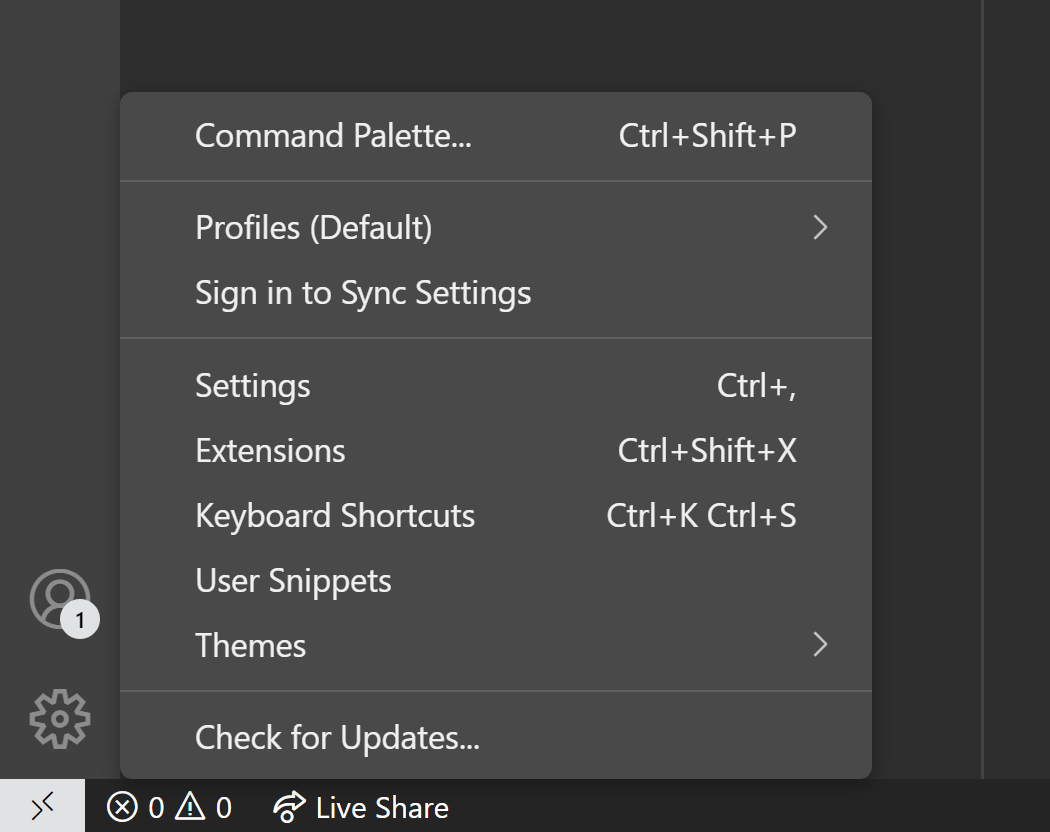
\includegraphics[scale=0.4]{settings_bottom_toolbar}
      \end{column}
      \begin{column}{0.4\textwidth}
        Open VSCode's settings through the bottom left Settings button.
      \end{column}
    \end{columns}
  \end{frame}
  \begin{frame}
    \frametitle{Changing VSCode's default terminal to Git Bash (cont.)}
    \begin{columns}[onlytextwidth]
      \begin{column}{0.4\textwidth}
        Change the Default terminal to Git Bash, as shown:
      \end{column}
      \begin{column}{0.6\textwidth}
        \centering
        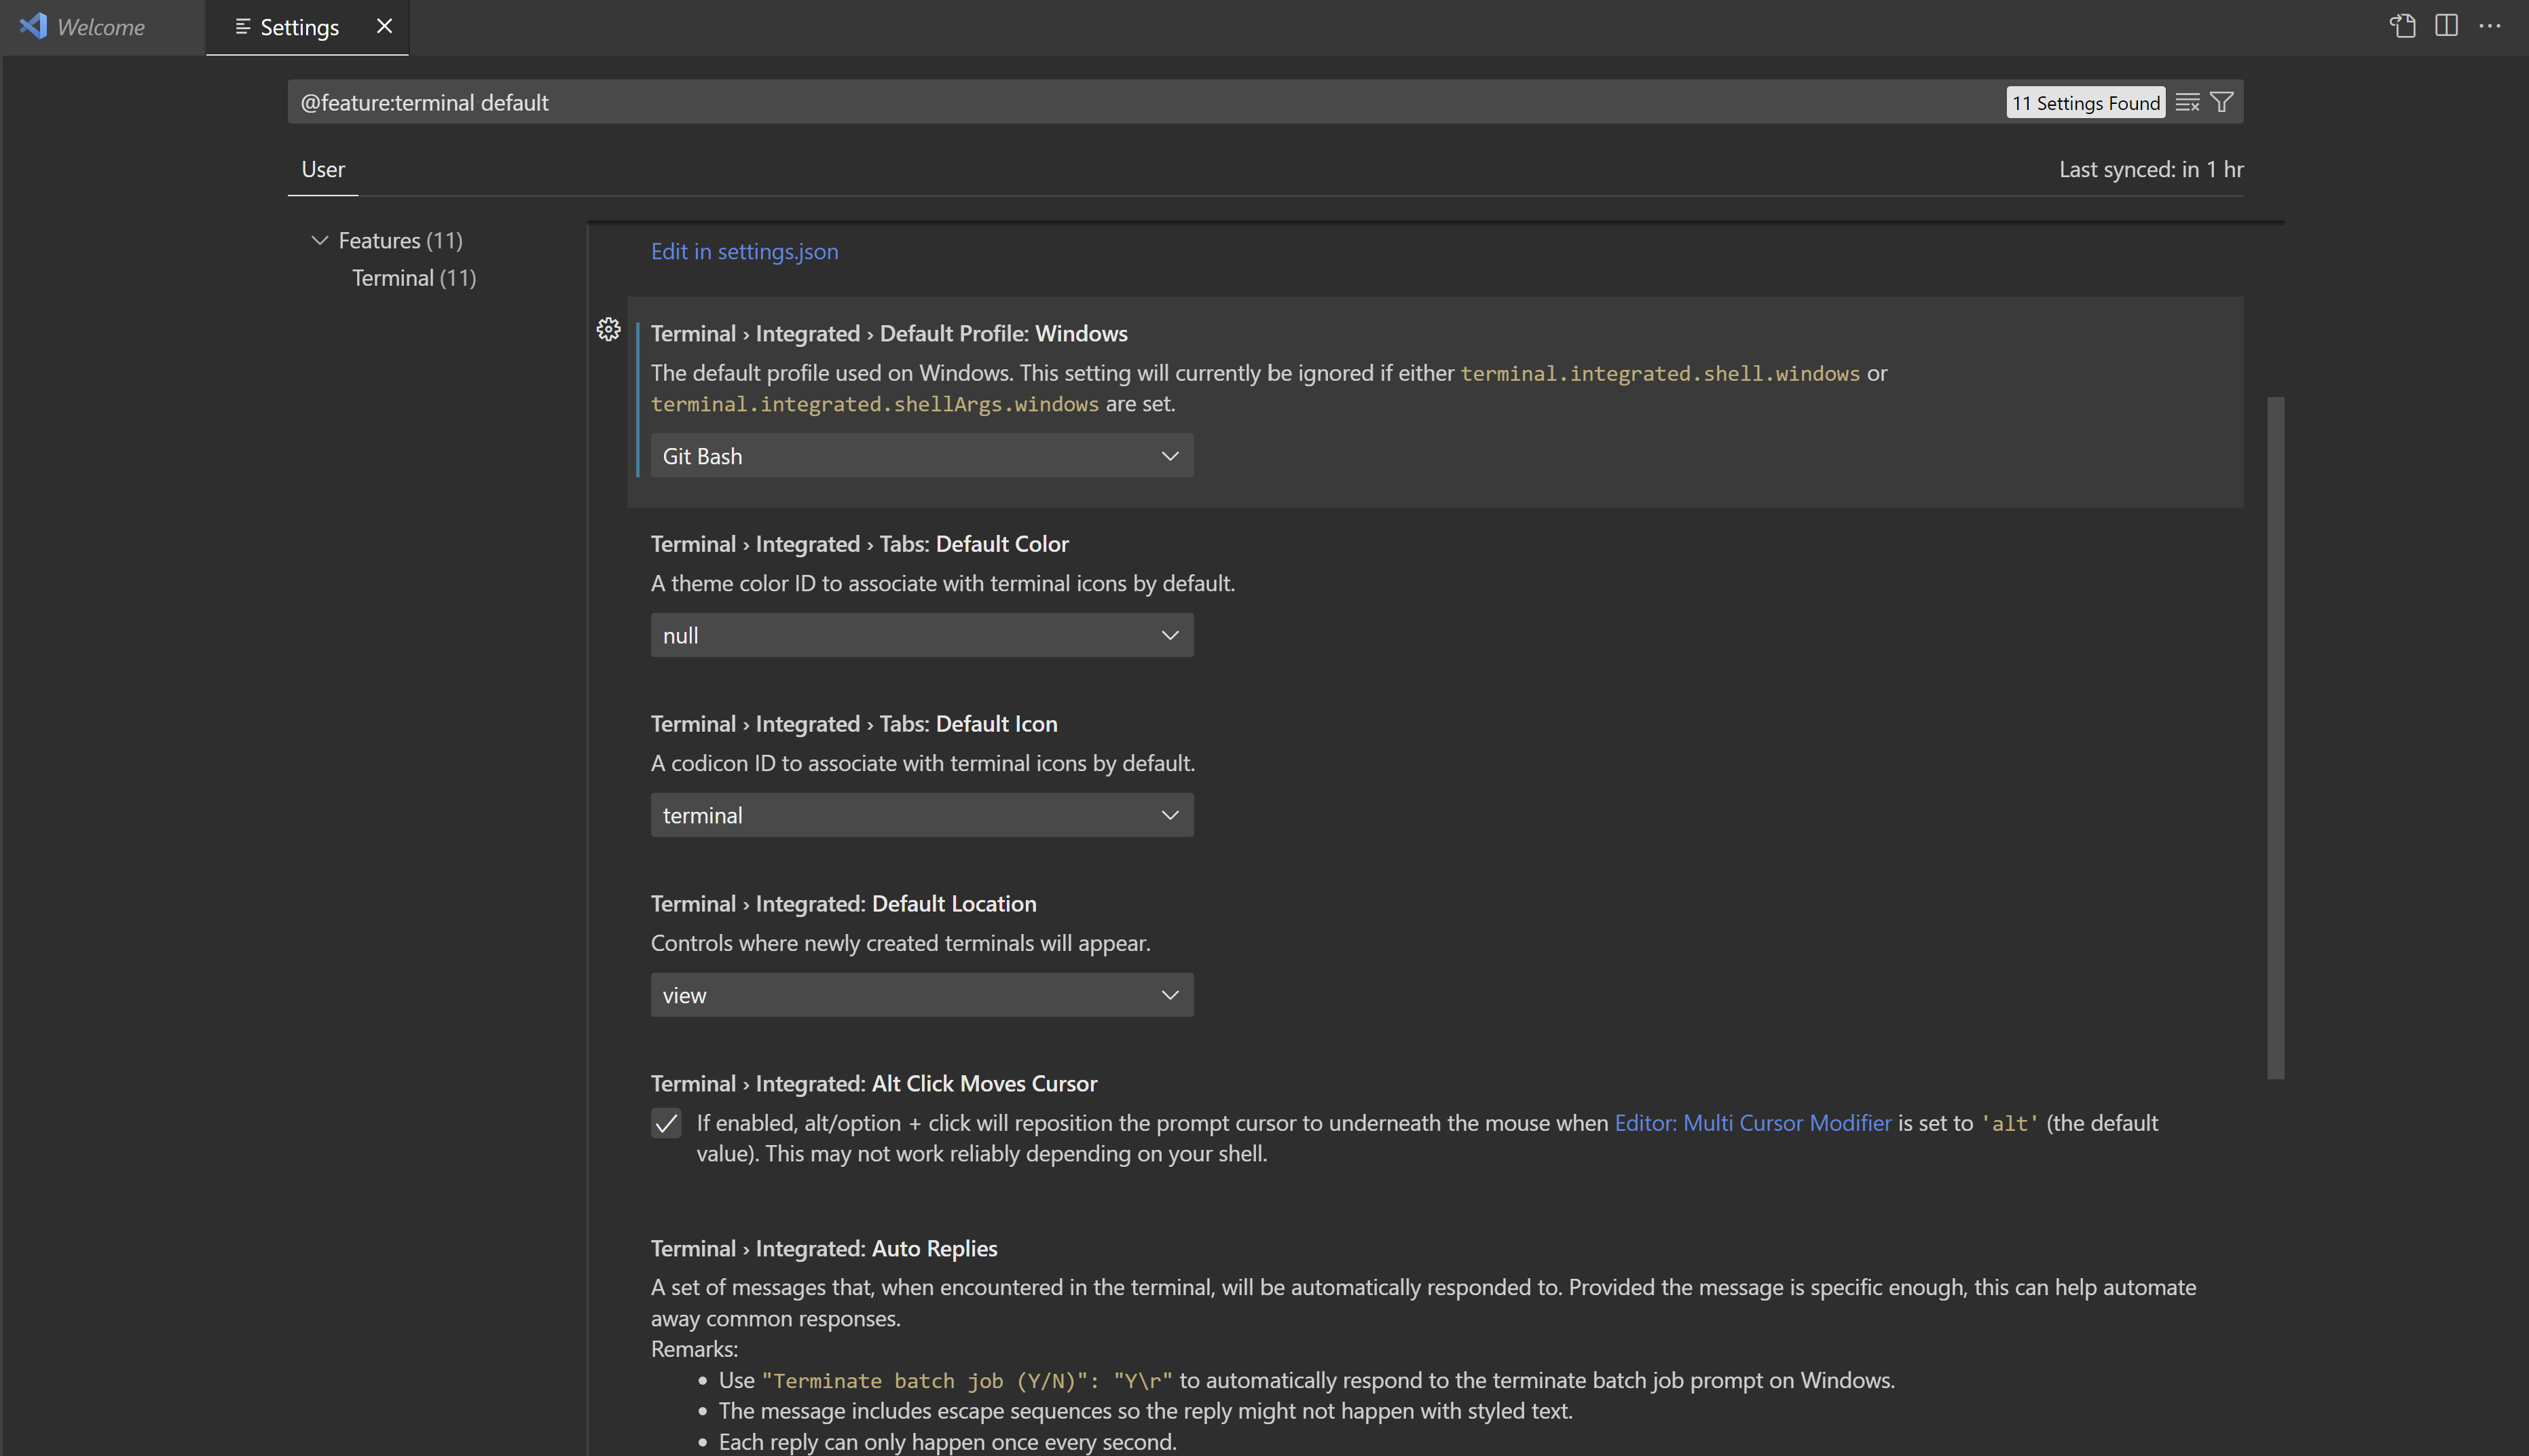
\includegraphics[scale=0.18]{default_terminal}
      \end{column}
    \end{columns}
  \end{frame}

  \begin{frame}
    \frametitle{Opening a Git Bash Terminal in VSCode}
    Now, open up a Terminal instance in VSCode from the top left toolbar.
    \vspace{0.5cm}

    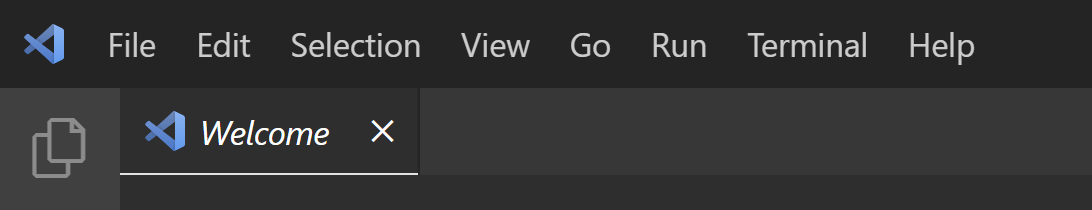
\includegraphics[scale=0.6]{terminal_toolbar}
  \end{frame}
  \begin{frame}
    \frametitle{Opening a Git Bash Terminal in VSCode (cont.)}
    You should now see a colorful terminal. 
    
    We will use VSCode's Terminal with Git Bash when referring to a `Terminal', unless otherwise stated.
    \vspace{0.5cm}  

    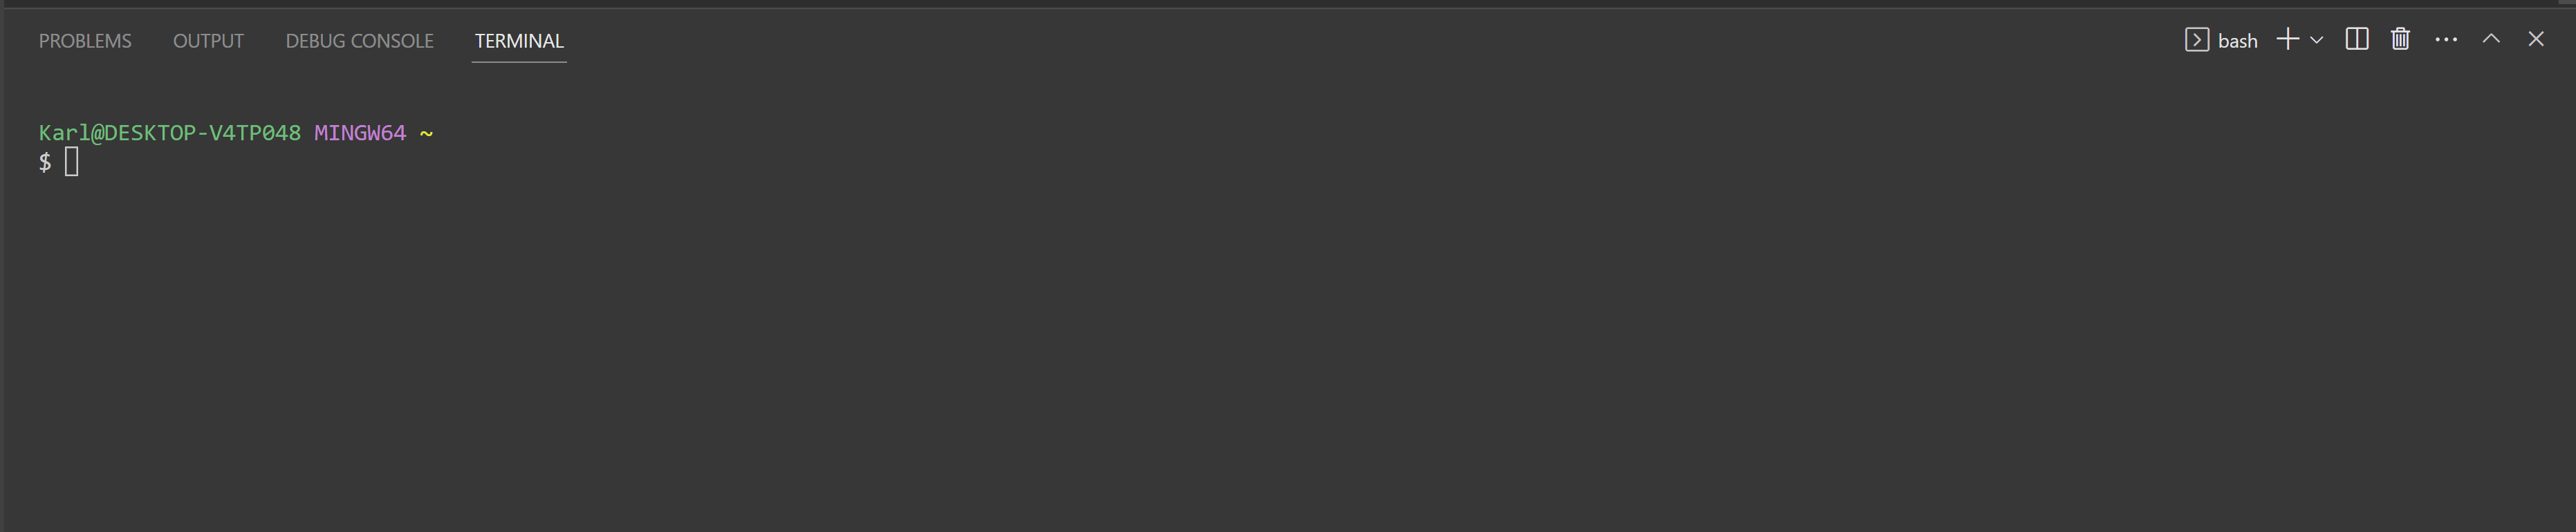
\includegraphics[scale=0.25]{terminal}
  \end{frame}


  \begin{frame}[fragile]
    \frametitle{Installing Yarn}

    Yarn is my preferred package manager, though there are others out there! Yarn will help us more efficiently handle external
    dependencies/libraries.

    In your Terminal, enter the following command:
    \newline
    \begin{bashcode}
$ npm install --global yarn
    \end{bashcode}

  \end{frame}

  \begin{frame}[fragile]
    \frametitle{Creating a React Native project with Expo}

    Expo allows us to run the app on iOS and Android using the Expo Go app. 

    In your Terminal, enter the following command:
    \newline
    \begin{bashcode}
$ yarn create expo-app myNewProject
    \end{bashcode}
    \vspace{0.5cm}
    Whichever directory you were in previously, you should now see a new folder /myNewProject created!
  \end{frame}

  \begin{frame}[fragile]
    \frametitle{Trying out React Native}

    Now that we have /myNewProject, let's run the app!

    Enter the following commands into your Terminal:
    \newline
    \begin{bashcode}
$ cd myNewProject/
$ yarn expo start
    \end{bashcode}
    \vspace{0.5cm}
    After a while a QR code should have popped up, scan it with the Expo Go app!
    If you're on iOS, you'll still need to have the Expo Go app but scan it with the Camera app instead.
  \end{frame}
  
  \appendix

  \begin{frame}[standout]
    End of Lesson

    {\small Questions? Reach out at:}
    {\footnotesize karlorjalo@gmail.com}
  \end{frame}

\end{document}